\documentclass[main.tex]{subfiles} % Subfile-Class


% ============================================================================== %
%                            Subfile document                                    %
% ============================================================================== %

\begin{document}

% Template

\subsubsection{Chassis und Fahrwerk}

Dieser Abschnitt beschreibt die Evaluierung des Fahrwerks sowie die
Konstruktion des Chassis. Dabei werden die Anforderungen an Gewicht, Kosten und
Funktionalität sowie die konstruktiven Entscheidungen im Detail erläutert.

% ===================================================================================
\subsubsection*{Anforderungen}

\textbf{Gewicht:} \newline
Das Gewicht stellt bei allen Baugruppen einen kritischen Faktor dar. Da
leistungsstarke Schrittmotoren und der Akku bereits einen Grossteil des
Gewichtsbudgets beanspruchen, verbleibt für das Chassis lediglich ein Budget von
200 Gramm. Dies erfordert eine leichte, aber dennoch stabile Konstruktion. Die
Gewichtsoptimierung wurde bereits in der frühen Planungsphase berücksichtigt, um
sicherzustellen, dass das Fahrzeug die Anforderungen hinsichtlich Stabilität und
Belastbarkeit erfüllt.

\textbf{Kosten:} \newline
Um die Kosten niedrig zu halten, soll auf die frei verfügbaren Ressourcen der
Hochschule Luzern zurückgegriffen werden. Das Team kann 25 Stunden Druckzeit am
HSLU-T\&A-Drucker sowie 1 Stunde Maschinenlaufzeit des Lasersystems kostenfrei
nutzen. Diese Ressourcen werden optimal ausgeschöpft, um den Einsatz von
Einkaufsteilen zu minimieren. Ziel ist es, das verfügbare Budget vor allem für
funktionskritische Baugruppen wie den Greifmechanismus und die Antriebssteuerung
einzusetzen.

% ===================================================================================
\subsubsection*{Chassiskonstruktion}

Das Chassis basiert auf einer 6 mm dicken Grundplatte aus MDF, einem leichten
und kostengünstigen Material. MDF bietet den Vorteil, dass es einfach zu
bearbeiten ist und alle notwendigen Ausschnitte präzise mit dem Lasersystem der
Hochschule gefertigt werden können. Abbildung~\ref{fig:Grundplatte} zeigt das
Design der Grundplatte des ersten Prototyps. Die Bauteilplatzierung ist
vorläufig und wird in PREN 2 voraussichtlich weiter optimiert. In dieser Phase
wird die Grundplatte auch mit zusätzlichen Aussparungen versehen, um weiteres
Gewicht einzusparen.

\begin{figure}[H]
    \centering
    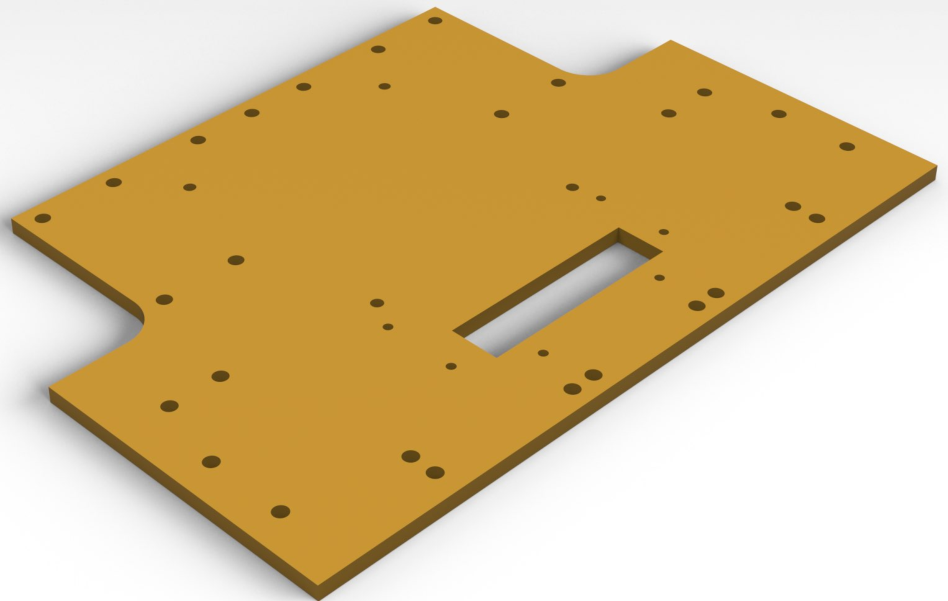
\includegraphics[width=0.6\textwidth]{Grundplatte.pdf}
    \caption{Grundplatte in Siemens NX}~\label{fig:Grundplatte}
\end{figure}

Abbildung~\ref{fig:Chassis_komplett} zeigt das Chassis mit allen Anbauteilen,
die mit dem 3D-Drucker gefertigt werden. Diese Konstruktion ist für
Prototypentests gedacht und daher nicht platzsparend ausgelegt. Sie ermöglicht
eine einfache Verkabelung der Leiterplattensowie den schnellen Austausch
einzelner Komponenten. Der modulare Aufbau erlaubt eine problemlose Anpassung
in PREN 2. Obwohl das aktuelle Design das Gewichtsbudget knapp überschreitet,
bestehen zahlreiche Möglichkeiten zur weiteren Optimierung. So ist geplant, die
Anbauteile mit Aussparungen zu versehen und mit einer Art Wabenstruktur
aufzubauen, um das Gewicht zu reduzieren, ohne die Stabilität zu
beeinträchtigen. Diese Strukturen sind besonders geeignet, da sie eine hohe
Festigkeit bei minimalem Materialeinsatz bieten und sich im 3D-Druck effizient
umsetzen lassen.

\begin{figure}[H]
    \centering
    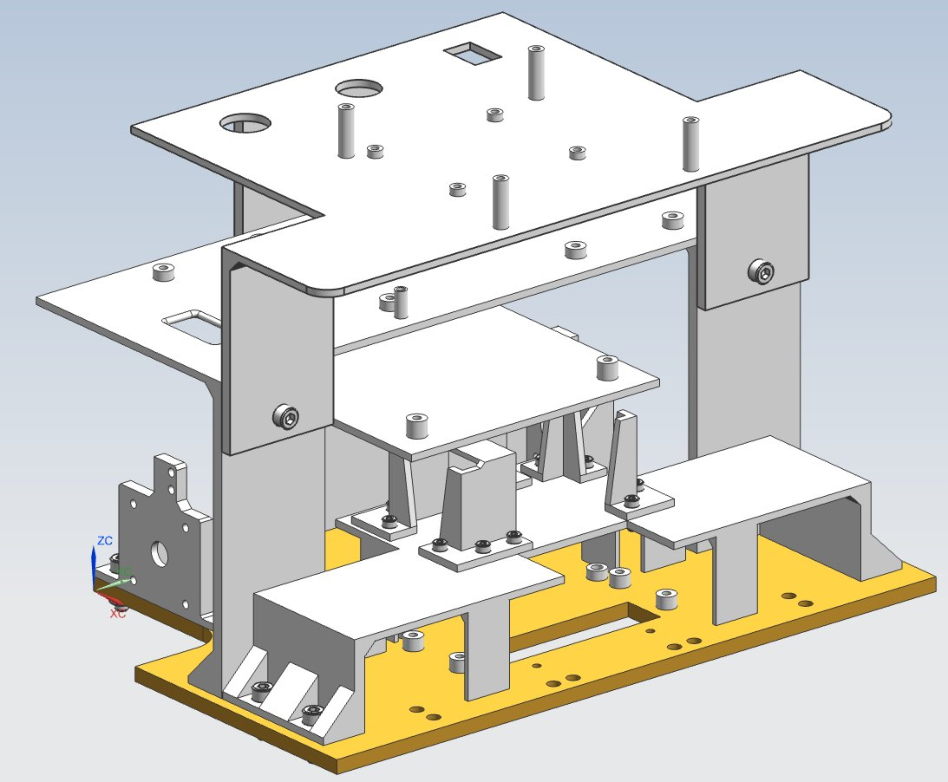
\includegraphics[width=0.75\textwidth]{Chassis_komplett.pdf}
    \caption{Chassis mit sämtlichen Anbauteilen in Siemens NX}~\label{fig:Chassis_komplett}
\end{figure}

\newpage

\subsubsection*{Fahrwerk}

Das Fahrwerk basiert auf einem Design mit zwei angetriebenen Rädern und einer
Laufkugel als drittem Auflagepunkt, um Stabilität zu gewährleisten. Diese
Lösung minimiert die Anzahl der Einkaufsteile und damit die Kosten. Zudem
bietet sie eine hohe Wendigkeit des Fahrzeugs. Abbildung~\ref{fig:Fahrwerk}
zeigt die Umsetzung mit den beiden Hinterrädern und der vorderen Laufkugel. Die
Platzierung der angetriebenen Räder an der Hinterachse ermöglicht präzise
Kurskorrekturen, da das Fahrzeug durch kleine Bewegungen der Hinterräder seine
Ausrichtung leicht ändern kann. Dies erlaubt es dem Fahrzeug, auf Knotenpunkten
effizient zu drehen und verschiedene Wegabzweigungen zu überprüfen.

\begin{figure}[H]
    \centering
    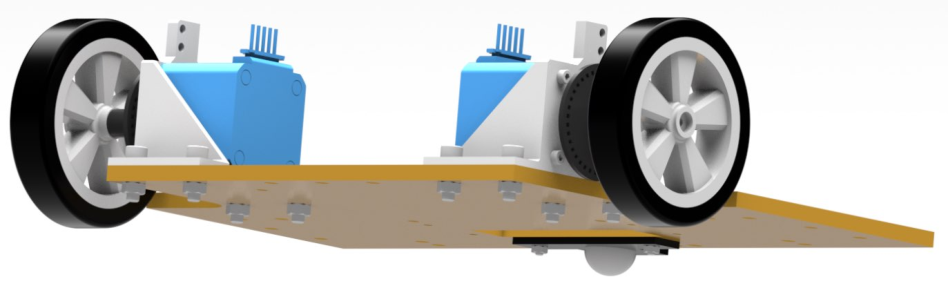
\includegraphics[width=0.75\textwidth]{Fahrwerk.pdf}
    \caption{Grundplatte mit Rädern und Laufkugel in Siemens NX}~\label{fig:Fahrwerk}
\end{figure}

Die Radgrösse wurde auf 80 mm festgelegt, wodurch eine maximale Geschwindigkeit
von 1,676~m/s erreicht wird. Die Berechnung erfolgt nach folgender Formel:

\[ v_{max} = n_{Motor} \cdot d_{Rad} \cdot \pi = 1.676 \, \frac{\text{m}}{\text{s}} \]

Die Räder vom Typ FIT0500 von DFRobot wurden über eine Sammelbestellung der
Hochschule Luzern beschafft, um die Umweltbelastung durch Lieferungen zu
reduzieren. Die endgültige Auswahl der Laufkugel steht noch aus. Vier
verschiedene Modelle wurden bestellt, die Tests und die finale Entscheidung
erfolgen jedoch erst in PREN 2, da ein Test ohne das komplette Fahrzeug nicht
aussagekräftig wäre. In dieser Phase werden auch die Auswirkungen der Laufkugel
auf das Fahrverhalten genauer untersucht, um sicherzustellen, dass das Fahrzeug
unter verschiedenen Bedingungen zuverlässig und stabil agiert.

\end{document}
